\chapter{Energy Reconstruction}
\label{sec:energy}
	The~second stage is the~reconstruction of the~particle's energy using a~fit of its reconstructed track (see Section~\ref{sec:track}). We have tested three ways of reconstructing the~energy. Fitting is done using the~MINUIT algorithm implemented in ROOT~\cite{ROOT}. \textcolor{red}{Cite some CERN article directly on MINUIT, can add a~section. Or is it done using MIGRAD? The circle and RK4 probably was.}
	
	The~\textbf{Cubic Spline Fit} was a~tested and later rejected method of energy reconstruction. It uses smoothly connected piecewise cubic polynomials between uniformly spaced nodes. The reconstructed energy is calculated using the~fit parameters by computing the~radius of curvature in different points of the~fitted curve using the~known magnitude of the~magnetic field perpendicular to the~trajectory. We rejected this method because the~tuning of the~fit turned out to be unpractical compared to the~other used methods. \textcolor{red}{Reconstructs energy at every position (even though the~actual energy doesn't change much) and it might be slower but no profiling has been done yet. Of course, it wasn't tested on the newer track reconstruction methods at all.}
	
	The~\textbf{Circle and Lines Fit} was chosen as an~alternative since this corresponds to the~shape of a~trajectory of a~charged particle crossing a~finite volume with a~homogeneous magnetic field. The~energy of the~particle can be estimated using the~fitted radius and the~magnitude of the~perpendicular magnetic field in the~middle of the~\ac{TPC}.
	
	The~\textbf{Runge-Kutta Fit} uses the~4th order Runge-Kutta numerical integration described in Section~\ref{sec:rks}. Initial parameters of the~track (including the~particle's energy) are optimized so that the~integrated trajectory fits to the~reconstructed one. This fit can also be performed as a~single parameter (i.e., energy) fit if we get the~initial position and orientation of the~particle on the~entrance to the~\ac{TPC} from previous detectors (\ac{Tpx3} and \ac{MWPC}, see Section~\ref{sec:IEAP}).
	
	\begin{figure}
		\centering
		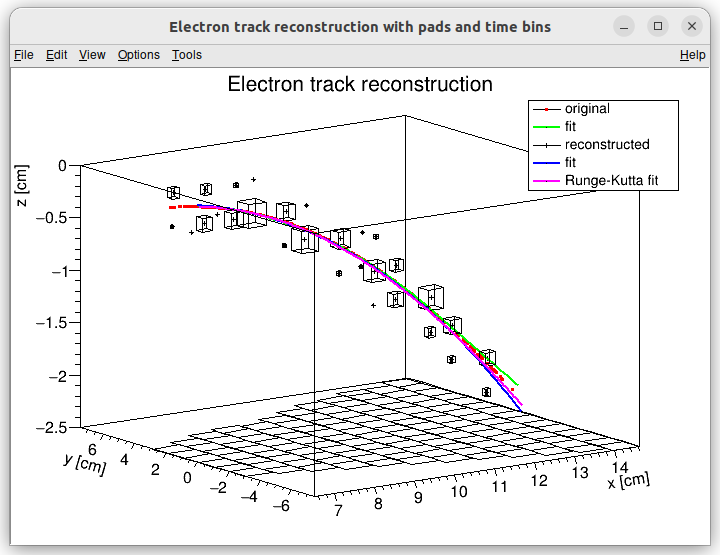
\includegraphics[width=0.5\textwidth]{9010_3d.png}
		\caption{Example of a~fitted reconstructed track. \textcolor{red}{Swap for better image.}}
		\label{fig:90103d}
	\end{figure}
	
	\section{Cubic Spline Fit}
	\label{sec:cspline}
		The~first attempt to get an~estimate of the~kinetic energy of the~particle uses a~cubic spline fit. We use an~electron track starting in the~origin of our coordinate system with an~initial direction in the~positive $x$~axis. The~ example track is simulated microscopically (see Section~\ref{sec:microsim}) with a~kinetic energy of 8~MeV in a~gas mixture 90\%~Ar~+~10\%~CO$_2$ (the~same track was used in Section~\ref{sec:trackfirst}). \textcolor{red}{This track should probably be described in the~simulation chapter.}
				
		In order to calculate the~spline, we use the~class \textit{TSpline3} from ROOT. This allows us to evaluate the~spline using the~coordinates $(x_n,z_n)$ of each node and the~derivatives $d_1,d_2$ in the~first and the~last node. We can fit these parameters of a~fixed amount of nodes to the~simulated trajectory. We use the~IMPROVE algorithm provided by the~\textit{TMinuit} class in ROOT (\textcolor{orange}{there are some guidelines for fonts in MFF UK template (Czech version) that I will eventually apply (see notes in the conclusion)}). This algorithm attempts to find a~better local minimum after converging (\textcolor{orange}{could reformulate a~bit, taken word for word from some manual}).
		
		After the~fit converges, we calculate an~energy estimate using the~radius of curvature, which we can extract from the~fitted spline equation at every point of the~trajectory. The~part of the~spline corresponding to a~given node is defined as
			\begin{equation}
				z(x) = z_n + b \Delta x+c(\Delta x)^2+d(\Delta x)^3,
			\end{equation}
		where $\Delta x = x-x_n$ and $b,c,d$ are coefficients. Using this equation, we derive the~radius of curvature\footnote{For the~general formula see \url{https://en.wikipedia.org/wiki/Curvature\#Graph_of_a_function}.} as:
			\begin{equation}
				r(x) = \frac{\left(1+z'^2(x)\right)^\frac{3}{2}}{z''(x)} = \frac{\left(1+\left(b+2c\Delta x+3d(\Delta x)^2\right)^2\right)^\frac{3}{2}}{2c+6d\Delta x}.
			\end{equation}
		Based on the~geometry of our~detector, we assume that the~magnetic field satisfies $\bm{B}(x,0,z) = (0,B(x,z),0)$ for a~track in the~XZ~plane. Since the~electron is relativistic, the~effect of the~electric field on its trajectory is negligible. The~Lorentz force $F_L$ is then always perpendicular to the~momentum of the~electron and acts as a~centripetal force $F_c$ (\textcolor{orange}{not quite sure how to handle this then?}):
			\begin{gather}
				\begin{aligned}
					\bm{F_L} &= \bm{F_c},\\
					\norm{e\bm{v}\times\bm{B}} &= \frac{\gamma m_e v^2}{r},\\
					e c\beta B &= \frac{E_{0e} \beta^2}{r\sqrt{1-\beta^2}},\\
					\sqrt{1-\beta^2} &= \frac{E_{0e} \beta}{ecBr},
				\end{aligned}\\
				\beta^2(x) = \left[1+\left(\frac{E_{0e}}{ecB(x,z(x))r(x)}\right)^2\right]^{-1}, \label{eq:ekin1}
			\end{gather}
		where $e$~is the~elementary charge, $c$~is the~speed of light in vacuum, $m_e$~is the~rest mass of electron, $E_{0e} = m_e c^2$ is its rest energy, $\gamma$~is the~Lorentz factor, $\bm{v}$~is the~velocity of the~electron, and $\beta = \frac{v}{c}$. The~kinetic energy for a~given point on the~trajectory is then given as
			\begin{equation}
				\label{eq:ekin2}
				E_\text{kin}(x) = \left(\frac{1}{\sqrt{1-\beta^2(x)}}-1\right)E_{0e}.
			\end{equation}
		We can then average these estimates at multiple points (\textcolor{red}{possibly using some weights to account for the~change in accuracy}, this wasn't optimized and we just ended with the graph) to get a~single value. This method was later rejected in favor of the~circle and lines fit \textcolor{orange}{the name was already established at the~beginning of the chapter} described in the~next section.
		\textcolor{red}{Add some figures.}
		
		\begin{figure}
			\centering
			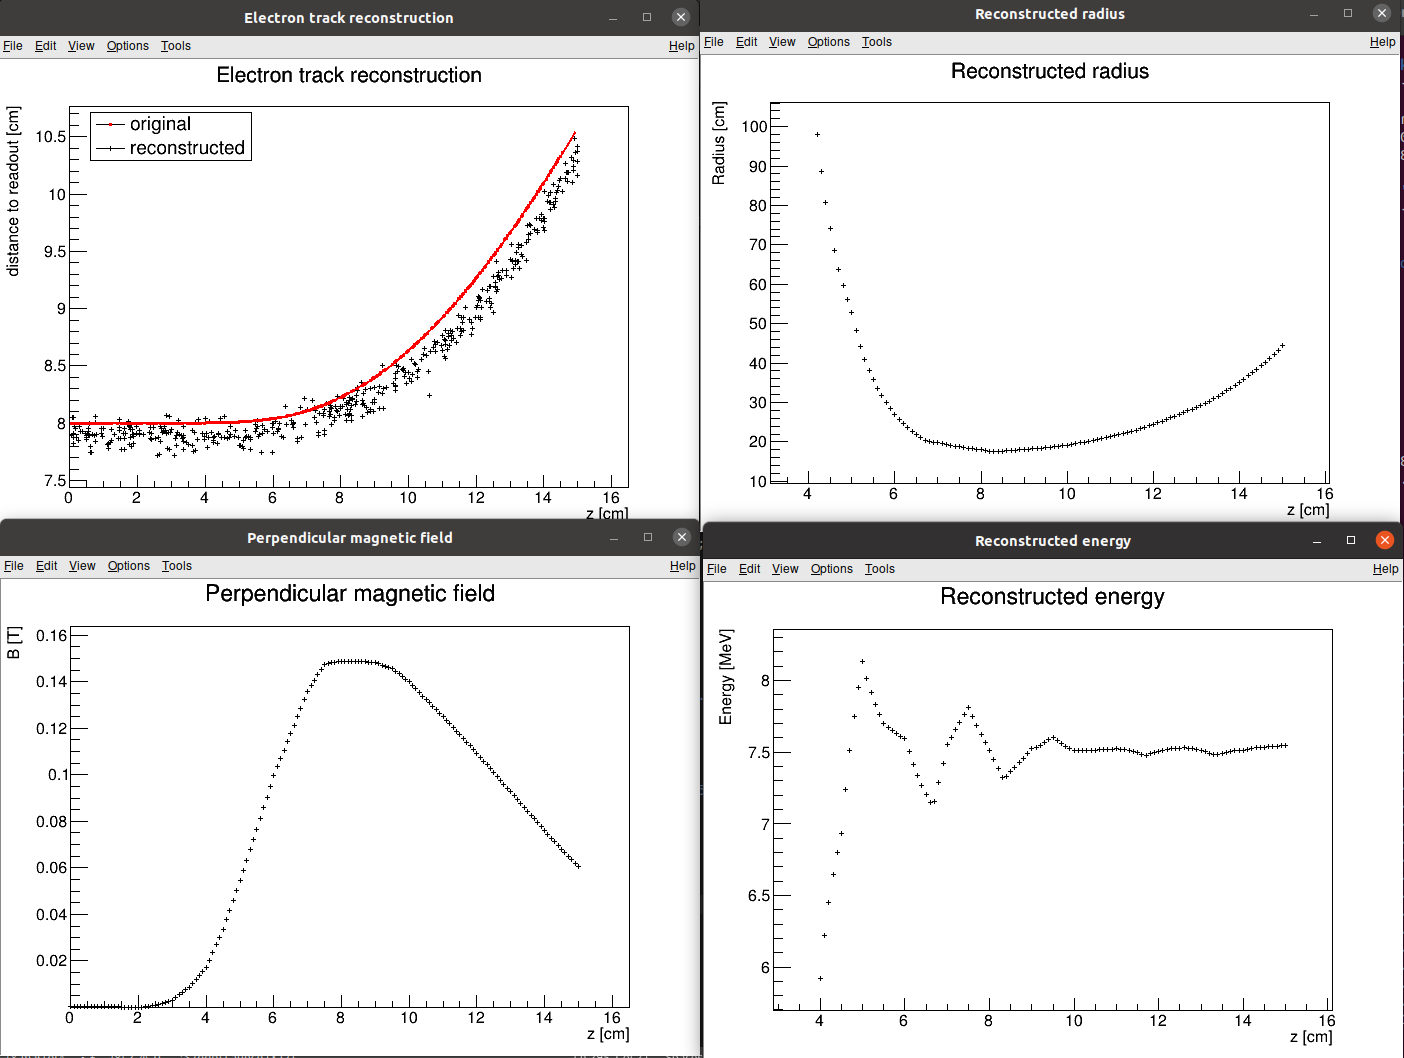
\includegraphics[width=0.8\textwidth]{9010_splines.png}
			\caption{First attempt at a~track reconstruction using only the~drift velocity. Spline energy reconstruction attempt. \textcolor{red}{Swap for better image(s) -- subfigure environment, correct coordinates.}}
			\label{fig:9010splines}
		\end{figure}
	
	\section{Circle and Lines Fit}
	\label{sec:clines}
		Another way to estimate the~particle's kinetic energy is to~fit its (\textcolor{orange}{??}) trajectory with a~circular arc with lines attached smoothly. This shape of trajectory corresponds to a~movement of a~charged particle through a~homogeneous magnetic field perpendicular to the~particle's momentum and limited to a~certain volume. In general, the~shape of such a~trajectory with a~non-perpendicularly oriented momentum is a~spiral. In our case, the~magnetic field is approximately toroidal and the~particle motion is nearly perpendicular to it (\textcolor{red}{verify, could add some magnetic field plots in different vertical planes; shouldn't have a big effect on the reconstructed radius anyway}). At first, we tested a~2D version of this fit, then we adapted it to 3D.
		
		The~field in our detector is not homogeneous, it is therefore not entirely clear what value of magnetic field should be used along with the~fitted radius (using equations~\ref{eq:ekin1} and~\ref{eq:ekin2}) to get the~best estimate for the~kinetic energy. Since we only use this method as the~first iteration of the~particle's energy that we later refine, an~optimal solution of this problem is not required. Instead, we tested two options: taking the~value of the~field in the~middle of the~fitted circular arc (\textcolor{red}{or is it in the middle $x$ of the OFTPC?}) and taking the~average field along it. \textcolor{red}{We haven't really tried to plot this for multiple tracks, but these estimates are saved somewhere and could be plotted.}
		
		\subsection{Two-dimensional fit}
			In the~2D case, the~fitted function used for the~electron track\footnote{Electron tracks bend towards negative~$z$, we need to use the~upper part of the~circle} described in Section~\ref{sec:cspline} (\textcolor{red}{or in microsim? one specific track at the time, technically this function doesn't work for a curvature that gets outside of the semicircle}) is defined as follows: \textcolor{red}{Maybe describe this track that we used at the~beginning somewhere earlier (section microscopic simulations \textrightarrow~Testing track?) so that it is easier to refer to it in multiple sections. It is not part of the~early GitHub commits, so maybe it won't be possible to create exact replicas of the~images, but they should be at least very similar.}
				\begin{equation}
					\label{eq:clines2d}
					z(x) = \begin{cases}
								a_1x+b_1 & x<x_1\\
								z_0+\sqrt{r^2-(x-x_0)^2} & x_1\leq x\leq x_2\\
								a_2x+b_2 & x>x_2
						   \end{cases},
				\end{equation}
			where $a_{1,2}$ and $b_{1,2}$ are the~parameters of the~lines, $(x_0,z_0)$ is the~center of the~circle, $r$ is its radius, and $(x_{1,2},z_{1,2})$ are the~coordinates of the~function's nodes. That means we have 9~parameters ($z_{1,2}$ are not used in the~function) along with 2~continuity conditions and 2~smoothness conditions (\textcolor{orange}{9~parameters of the described function, 5~of them independent after taking the conditions into account}). For the~fit, we use the~coordinates of the~nodes and the~radius of the~circle, which gives us 5~independent parameters (only the~radius has to be larger than half of the~distance between nodes). The~continuity conditions (combined with the~relations for $z_{1,2}$) are
				\begin{equation}
					\label{eq:ccont}
					z_{1,2} = a_{1,2}x_{1,2}+b_{1,2} = z_0-\sqrt{r^2-(x_{1,2}-x_0)^2},
				\end{equation}
			the~smoothness conditions are
				\begin{equation}
					\label{eq:a12}
					a_{1,2} = \frac{x_0-x_{1,2}}{\sqrt{r^2-(x_{1,2}-x_0)^2}}.
				\end{equation}
			Together with the Equation~\ref{eq:ccont} we get the~values of $b_{1,2}$
				\begin{equation}
					\label{eq:b12}
					b_{1,2} = z_{1,2} - a_{1,2} x_{1,2}.
				\end{equation}
			For the~coordinates of the~center of the~circle, we can use the~fact that the~center has to lie on the~axis of its chord. In other words, there is a~value of a~parameter~$t$ such that, using the~parametric equation of the~axis
				\begin{equation}
					\begin{pmatrix} x_0\\ z_0 \end{pmatrix} = \begin{pmatrix} \frac{x_1+x_2}{2}\\ \frac{z_1+z_2}{2} \end{pmatrix} + t \begin{pmatrix} \frac{z_2-z_1}{2}\\ \frac{x_1-x_2}{2} \end{pmatrix}.
				\end{equation}
			At the~same time, the~center has to be in a~distance of $r$ from the~nodes:
				\begin{gather}
					(x_1-x_0)^2 + (z_1-z_0)^2 = r^2,\notag\\
					\left(\frac{x_1-x_2}{2}+\frac{z_1-z_2}{2}t\right)^2 + \left(\frac{z_1-z_2}{2}+\frac{x_2-x_1}{2}t\right)^2 = r^2,\notag\\
					\left(\left(\frac{x_2-x_1}{2}\right)^2+\left(\frac{z_2-z_1}{2}\right)^2\right)t^2+\left(\frac{x_2-x_1}{2}\right)^2+\left(\frac{z_2-z_1}{2}\right)^2-r^2=0.
				\end{gather}
			Since our electron track bends towards negative $z$ and $x_2 > x_1$, we only care about the~solution with $t>0$
				\begin{gather}
					t = \sqrt{\frac{r^2}{\left(\frac{x_2-x_1}{2}\right)^2+\left(\frac{z_2-z_1}{2}\right)^2}-1},\\
					\begin{aligned}
						x_0 = \frac{x_1+x_2}{2} + \frac{z_2-z_1}{2} \sqrt{\frac{r^2}{\left(\frac{x_2-x_1}{2}\right)^2+\left(\frac{z_2-z_1}{2}\right)^2}-1},\label{eq:xz0}\\
						z_0 = \frac{z_1+z_2}{2} - \frac{x_2-x_1}{2} \sqrt{\frac{r^2}{\left(\frac{x_2-x_1}{2}\right)^2+\left(\frac{z_2-z_1}{2}\right)^2}-1}.
					\end{aligned}
				\end{gather}
			The~function defined in Equation~\ref{eq:clines2d} along with equations~\ref{eq:a12}, \ref{eq:b12}, and \ref{eq:xz0} derived using the~continuity and smoothness conditions (combined with the~relations for $z_{1,2}$) fully define our fitted function with parameters $r,x_{1,2},z_{1,2}$. \textcolor{red}{Some pictures of the~fit on the~tested track. Results of the~fit. Again, the~actual fit uses 8-z. Use GeoGebra schematics to generate a~picture of 2D geometry.}
			
			\begin{figure}
				\centering
				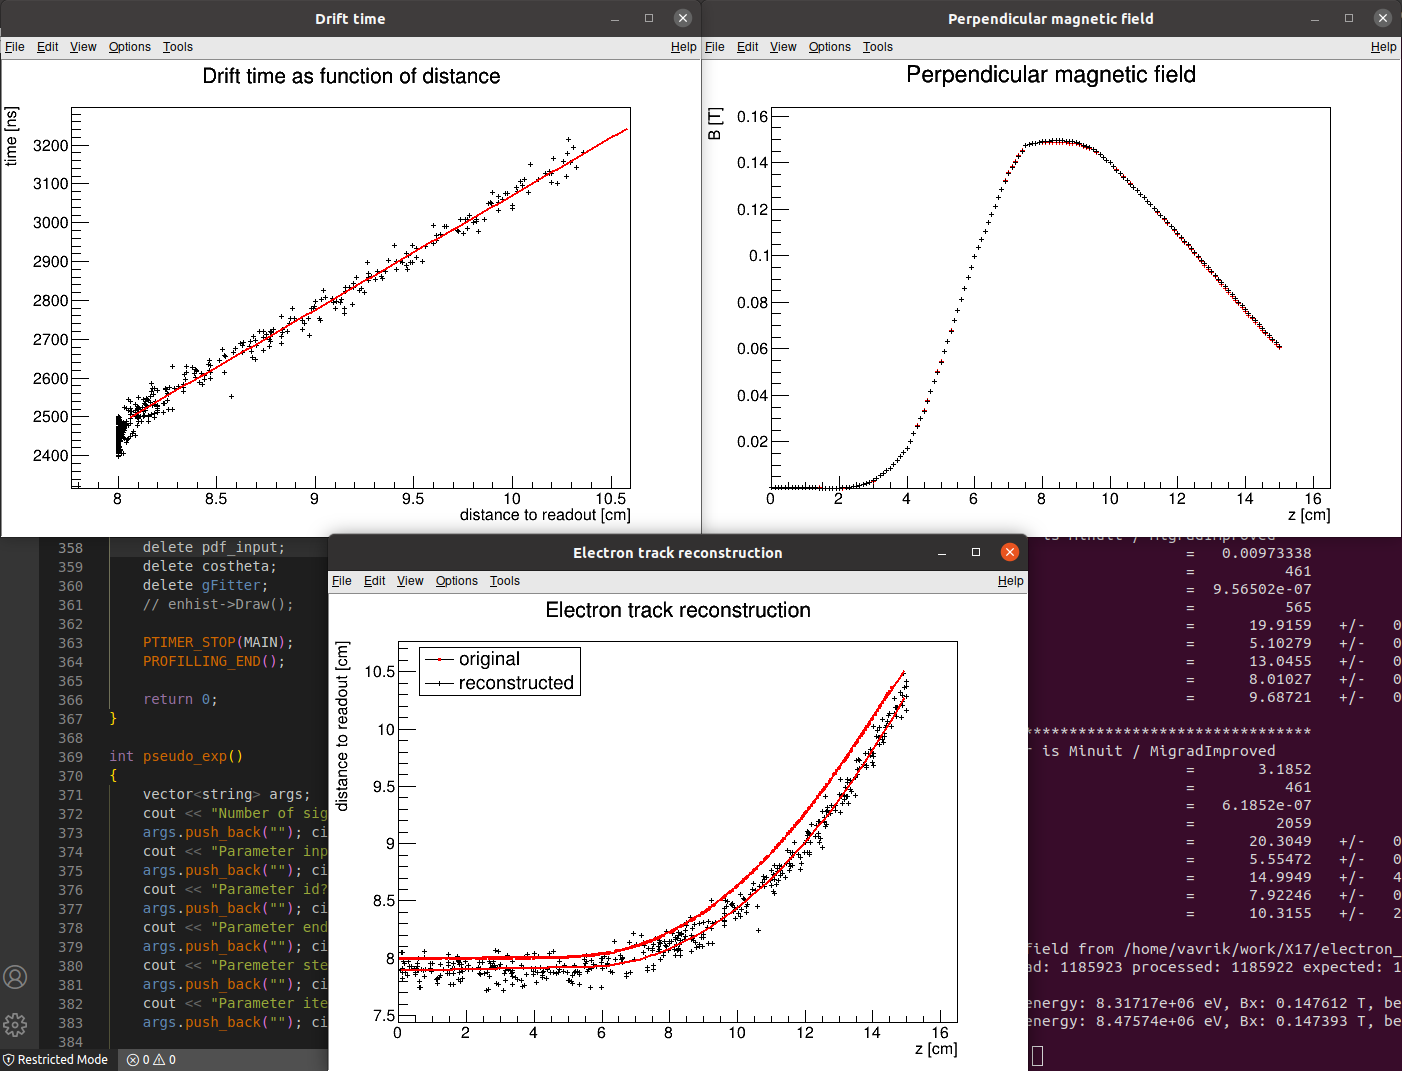
\includegraphics[width=0.8\textwidth]{9010_circle2D.png}
				\caption{First attempt at a~track reconstruction using only the~drift velocity. Circle and Lines Fit in 2D. \textcolor{red}{Swap for better image, correct coordinates.} \textcolor{orange}{Bias should be described in the previous chapter, not here.}}
				\label{fig:9010circle2D}
			\end{figure}
		
		\subsection{Three-dimensional fit}
			\textcolor{red}{Explain the geometry and least square method used for the~3D fit. Tested on a~Runge-Kutta sample, and with microscopic tracks + map simulation.}
			
			In three dimensions, the~shape of a~trajectory of a~charged particle in a~uniform magnetic field is a~cylindrical helix. Nevertheless, since we assume that the field is approximately perpendicular to the~particle's momentum at all times, we will further approximate the~trajectory with a~circular arc (with lines attached smoothly).
			
			We assume that the~initial position $\mathbf{X}_0 = (x_0,y_0,z_0)$ and direction $\theta,\varphi$ (\textcolor{red}{spherical angles as in Section~\ref{sec:coor}}) are known, since this information will be provided by \ac{Tpx3} and \ac{MWPC} layers. \textcolor{red}{We could further refine it at the~end of the current algorithm with some kind of global fit (all detector layers).} The fit then has four free parameters (\textcolor{red}{figure}):
				\begin{itemize}[nosep]
					\item the length of the first line $l$ (as measured from the initial position),
					\item the radius of the circular arc $r$,
					\item the central angle of the arc $\phi_\text{max} \in [0,2\pi]$,
					\item the direction of the curvature given by the angle $\alpha \in [0,2\pi]$ (right-handed with respect to the particle direction, $\alpha = 0$ if the particle curves towards negative~$z$ in a~plane given by~$\hat{z}$ and the direction vector).
				\end{itemize}
			Using these parameters, we can derive a parametrization of the~whole curve. Let $\mathbf{v}$ be the initial unit direction vector, i.e., using the spherical angles
				\begin{equation}
					\mathbf{v} = (\cos\varphi\cos\theta, \,\sin\varphi\cos\theta, \,\sin\theta)^\mathrm{T},
				\end{equation}
			then we can parameterize the first line as follows:
				\begin{equation}
					\mathbf{X}_\text{L1}(t) = \mathbf{X}_0 + t\mathbf{v} \quad t\in[0,l].
				\end{equation}
			This gives us the starting point of the~arc
				\begin{equation}
					\mathbf{X}_1 = \mathbf{X}_\text{L1}(l) = \mathbf{X}_0 + l\mathbf{v}.
				\end{equation}
			The vector $\mathbf{c}_1$ that lies in the~plane of curvature and points from $\mathbf{X}_1$ to the~center of curvature can be calculated using a composition of rotations. First, we rotate $\mathbf{v}$ to point in the~$\mathbf{\hat{x}}$ direction, the normal for $\alpha = 0$ than points in the $-\mathbf{\hat{z}}$ direction, we apply the $\alpha$ rotation and reverse the rotations into the~$\mathbf{\hat{x}}$ direction: \textcolor{orange}{(parameters are explained in the bullet points above)}
				\begin{equation}
					\begin{aligned}
						\mathbf{c}_1 &= R_z(\varphi)R_y(-\theta)R_x(\alpha)R_y\left(\frac{\pi}{2}\right)R_y(\theta)R_z(-\varphi)\mathbf{v},\\
						&= R_z(\varphi)R_y(-\theta)R_x(\alpha)(-\mathbf{\hat{z}}),\\
						&= \scalebox{0.95}{$
								\begin{pmatrix}
									\cos\varphi & -\sin\varphi & 0\\
									\sin\varphi & \cos\varphi & 0\\
									0 & 0 & 1
								\end{pmatrix}
								\begin{pmatrix}
									\cos\theta & 0 & -\sin\theta\\
									0 & 1 & 0\\
									\sin\theta & 0 & \cos\theta
								\end{pmatrix}
								\begin{pmatrix}
									1 & 0 & 0\\
									0 & \cos\alpha & -\sin\alpha\\
									0 & \sin\alpha & \cos\alpha
								\end{pmatrix}
								\begin{pmatrix}
									0\\ 0\\ -1
								\end{pmatrix}
							$},\\
						&= 	\begin{pmatrix}
								-\sin\alpha\sin\varphi+\cos\alpha\cos\varphi\sin\theta\\
								\phantom{-}\sin\alpha\cos\varphi+\cos\alpha\sin\varphi\sin\theta\\
								-\cos\alpha\cos\theta
							\end{pmatrix}.
					\end{aligned}
				\end{equation}
			\textcolor{orange}{Signs should be correct because right-handed rotation around $y$ rotates $z$ into $x$ and this one is the opposite.} \textcolor{red}{Seems like in this part of the~code $\theta$ is actually taken from the~pole. Instead of the~equator plane.} Similarly by rotating $\mathbf{\hat{y}}$, we can get the~normal vector $\mathbf{n}=\mathbf{v}\cross\mathbf{c}_1$ perpendicular to the~plane of the~trajectory:
				\begin{equation}
					\mathbf{n} = R_z(\varphi)R_y(-\theta)R_x(\alpha)\mathbf{\hat{y}}=
									\begin{pmatrix}
										-\cos\alpha\sin\varphi-\sin\alpha\cos\varphi\sin\theta\\
										\phantom{-}\cos\alpha\cos\varphi-\sin\alpha\sin\varphi\sin\theta\\
										\sin\alpha\cos\theta
									\end{pmatrix}.
				\end{equation}
			This allows us to express the coordinates of the~center $\mathbf{C}$ of the~circular arc:
				\begin{equation}
					\mathbf{C} = \mathbf{X}_1+r\mathbf{c}_1.
				\end{equation}
			We can then get the parametrization and the endpoint of the~circular arc using Rodrigues' rotation formula: (\textcolor{orange}{all parameters explained in the bullet points above})
				\begin{gather}
					\begin{aligned}
						\mathbf{c}_2 &= \mathbf{c}_1\cos\phi_\text{max} + (\mathbf{n}\cross\mathbf{c}_1)\sin\phi_\text{max} + \mathbf{n}(\mathbf{n}\cdot\mathbf{c}_1)(1-\cos\phi_\text{max}),\\
						&= \mathbf{c}_1\cos\phi_\text{max} - \mathbf{v}\sin\phi_\text{max},
					\end{aligned}\\
					\mathbf{X}_C(\phi) = \mathbf{C} - r(\mathbf{c}_1\cos\phi - \mathbf{v}\sin\phi) \quad \phi\in[0,\phi_\text{max}],\\
					\mathbf{X}_2 = \mathbf{X}_C(\phi_\text{max}) = \mathbf{C} - r\mathbf{c}_2,
				\end{gather}
			and if we define the~direction vector of the~second line, we also get its parametrization
				\begin{gather}
					\mathbf{w} = \mathbf{v}\cos\phi_\text{max} + (\mathbf{n}\cross\mathbf{v})\sin\phi_\text{max} = \mathbf{v}\cos\phi_\text{max} + \mathbf{c}_1\sin\phi_\text{max},\\
					\mathbf{X}_\text{L2}(s) = \mathbf{X}_2 + s\mathbf{w} \quad s\in[0,\infty).
				\end{gather}
				
			The fit is performed as a~(weighted) least square minimization (\textcolor{red}{MIGRAD ROOT}), therefore we need to derive the~distance of any point~$\mathbf{P}$ to the~fitted curve. For the first line, we simply compute the parameter value of the~closest point on the line:
				\begin{equation}
					\label{eq:segdist}
					\begin{aligned}
						t_P &= \mathbf{v}\cdot(\mathbf{P}-\mathbf{X}_1),\\
						d_{P1} &= \norm{\mathbf{P}-\mathbf{X}_\text{L1}(t_P)}.
					\end{aligned}
				\end{equation}
			If the parameter value is outside of its bounds defined above, we take the boundary value instead. The distance to the~second line is computed likewise. For the~circular arc (\textcolor{orange}{specific circular arc in the fit}), we find the closest point (\textcolor{orange}{on the arc}) by projecting the~center connecting line onto the~arc plane:
				\begin{gather}
					\mathbf{X}_{PC} = \mathbf{X}_C + r\frac{(\mathbf{P-\mathbf{X}_C})-(\mathbf{n}\cdot(\mathbf{P-\mathbf{X}_C}))\mathbf{n}}{\norm{(\mathbf{P-\mathbf{X}_C})-(\mathbf{n}\cdot(\mathbf{P-\mathbf{X}_C}))\mathbf{n}}},\\
					d_{PC} = \norm{\mathbf{P}-\mathbf{X}_{PC}}
				\end{gather}
			\textcolor{red}{Potential problem in the implementation -- might not be correctly handling $\phi$ out of bounds, the distance could be sometimes underestimated because of this.} The~shortest distance out of $d_{P1},d_{PC},d_{P2}$ is then taken as the distance to the~curve. \textcolor{red}{When calculating energy with the average field, only the arc is considered. Middle field in the current implementation taken in the middle~$x$ plane (intersection with the curve). TVirtualFitter+MIGRAD, maximal num of iterations, toleration. Different uncertainties in $x,y,z$ not taken into account.}
			
			\begin{figure}
				\centering
				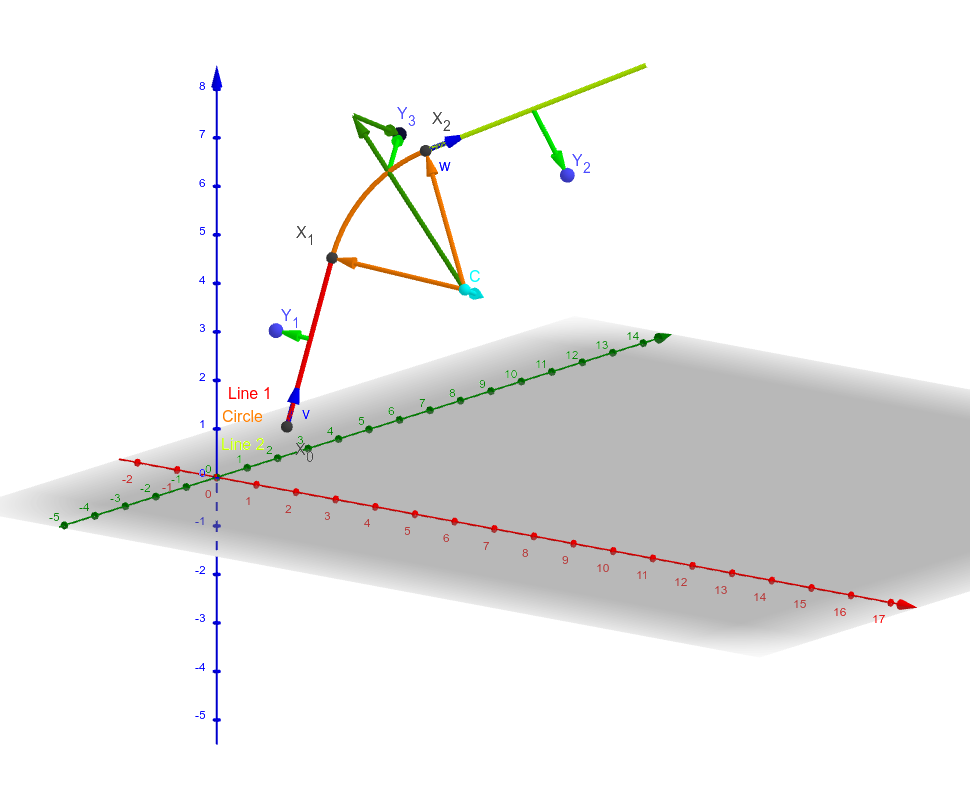
\includegraphics[width=0.8\textwidth]{circlefit.png}
				\caption{Circle and Lines Fit 3D geometry. \textcolor{red}{Swap for better image.}}
				\label{fig:circlefit}
			\end{figure}
	
	\section{Runge-Kutta Fit}
		The~Runge-Kutta fit uses the~\acf{RK4} numerical integration of the~equation of motion (see Section~\ref{sec:rks}) to find the~best values of the~track parameters -- the~track origin, initial velocity direction and the~kinetic energy. In order to speed up the~energy reconstruction, an~initial guess of these parameters can be obtained from the~3D circle fit described in the~previous section. Furthermore, assuming we know the track origin and orientation, we can perform a~single parameter fit of the~kinetic energy (\textcolor{red}{do some profiling and show that it is faster -- below in the microscopic testing}).
		
		The~fit is performed as a~least square minimization of the (weighted) distances of the~track points (true ionization vertices from the simulation or reconstructed points). The simulated \ac{RK4}~track consists of line segments with known endpoints, therefore we can calculate the distance of a~point from this segment analogically to Equation~\ref{eq:segdist} with $\mathbf{v}$ given as a~unit vector in the~direction of the segment.
		
		We need to find the~segment with the~lowest distance. We assume, that the~distance $d_\mathbf{P}(\tau)$ of a~point $\mathbf{P}$ to the point on the~track $\mathbf{X}(\tau)$ has a~single minimum (local and global), no local maximum (except the~interval endpoints) and no~saddle point
			\begin{equation}
				\label{eq:rk_assum}
				\exists!\tau_\text{min}\in[0,\tau_N]\colon\ \left(\forall\tau\in[0,\tau_N]\colon  d_{\mathbf{P}}(\tau) \geq d_{\mathbf{P}}(\tau_\text{min})\right)\ \lor\ \dv{d_{\mathbf{P}}}{\tau}{(\tau_\text{min})} = 0,
			\end{equation}
		where $N$ is the~number of \ac{RK4} steps. This is a~reasonable assumption for a~track with an~approximate shape of a~circular arc with a~radius $r$, since the~distance $d$ from a~point $\mathbf{C}$ on the~corresponding circle of a~point $\mathbf{P}$ offset by~$a$ from the~arc plane and by~$b$ from the~arc's center when projected on its plane is given by the law of cosines:
			\begin{equation}
				\label{eq:rkdemo}
				d^2 = a^2+b^2+r^2 - 2br\cos\alpha,
			\end{equation}
		where $\alpha$ is the~angle between points~$\mathbf{C}$ and~$\mathbf{P}$ as seen from the~center of the~arc (see Figure~\ref{fig:rkdemo}). This function is strictly convex for $\alpha\in\left(-\frac{\pi}{2},\frac{\pi}{2}\right)$ and in our case, the~center of the~arc lies outside of the~detector and $\alpha$ is restricted to a~small interval around zero (\textcolor{red}{especially considering that the initial guess should make the fitted trajectory reasonably close to any relevant point, in the~worst-case scenario, the~distance is overestimated which should keep the~fit from converging to such solutions}).
		
		\begin{figure}
			\centering
			\begin{subfigure}[t]{0.7\textwidth}
				\centering
				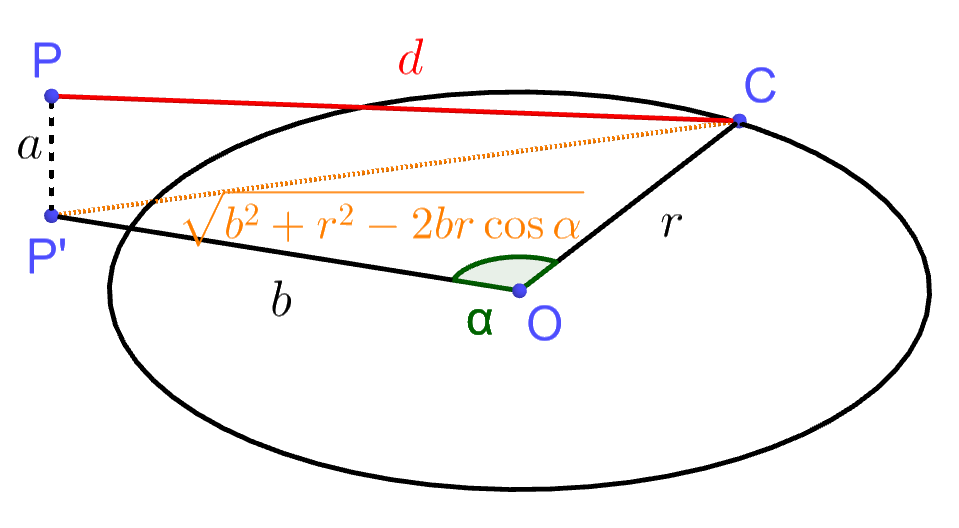
\includegraphics[width=\textwidth]{rk_circle_demo.png}
			\end{subfigure}
			\hfill
			\begin{subfigure}[t]{0.29\textwidth}
				\centering
				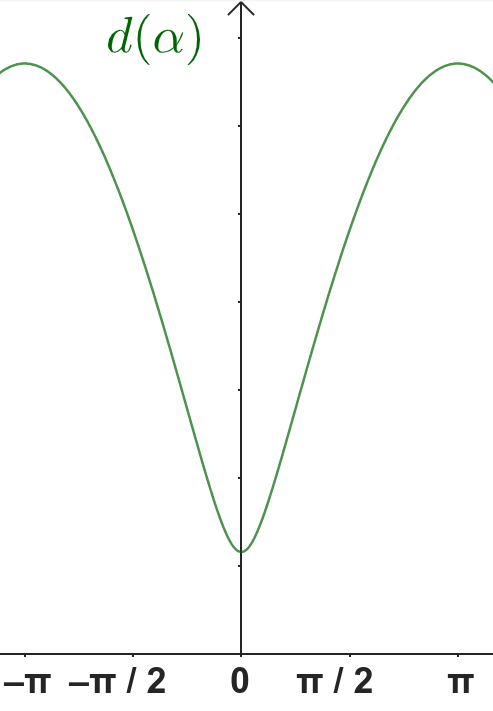
\includegraphics[width=\textwidth]{rk_circle_demo2.png}
			\end{subfigure}
			\caption{Demonstration of the~convexity of the~distance function $d(\alpha)$ for a~circular track (see Equation~\ref{eq:rkdemo}).}
			\label{fig:rkdemo}
		\end{figure}
		
		In a~more general case, if we consider the~vector $\mathbf{a}(\tau) = \mathbf{P}-\mathbf{X}(\tau)$ whose size is $\norm{\mathbf{a}(\tau)} = d_\mathbf{P}(\tau)$, then the~we get
			\begin{equation}
				2d_{\mathbf{P}}\dv{d_{\mathbf{P}}}{\tau}= \dv{d^2_{\mathbf{P}}}{\tau} = \dv{}{\tau} \sum_i a_i^2 = 2\sum_i a_i\dv{a_i}{\tau} = 2\mathbf{a}\cdot\dv{\mathbf{a}}{\tau} = -2\mathbf{a}\cdot\dv{\mathbf{X}}{\tau},
			\end{equation}
		therefore for the~derivative of~$d_\mathbf{P}(\tau)$ to be zero, $\mathbf{a}(\tau)$ has to be perpendicular to the~tangent of the~track. In 3D, for a~given $\mathbf{X}(\tau)$, this condition restricts $\mathbf{P}$ to a~plane. This means that for a~curving track we can find a~point~$\mathbf{P}$ for any two points $\mathbf{X}(\tau),\mathbf{X}(\sigma)$ with non-parallel tangents that has $\dv{d_{\mathbf{P}}}{\tau}{(\tau)} = \dv{d_{\mathbf{P}}}{\tau}{(\sigma)} = 0$, which violates the~assumption~\ref{eq:rk_assum}. If we have a~circle-and-lines track as described in the~previous sections, such a~point has to lie outside of the circular sector given by the~arc.
		
		For a~planar track, the envelope of all its normals is the~evolute of the curve (i.e., the~set of centers of all its osculating circles). If the~track has a~monotonous tangent angle
			\begin{equation}
				\alpha(\tau) = \atan{\frac{\dv{X_2}{\tau}}{\dv{X_1}{\tau}}}
			\end{equation}
		with minimal and maximal $\alpha$ differing by less than~$\pi$ (i.e., the~track changes direction by less than $180^\circ$), then all intersections of the~track's normals must lie on the~side of the~evolute closer to the track (\textcolor{red}{not obvious?, sometimes the sides are opposite?}). At the~same time, the~intersection must lie in the half planes given by the~normals at the~beginning and the~end of the~curve and pointing away from the~curve. Together, these three boundaries define a closed shape that will lie outside of the~\ac{OFTPC} for a~typical track in our detector.
			\begin{figure}
				\centering
				\begin{subfigure}[t]{0.49\textwidth}
					\centering
					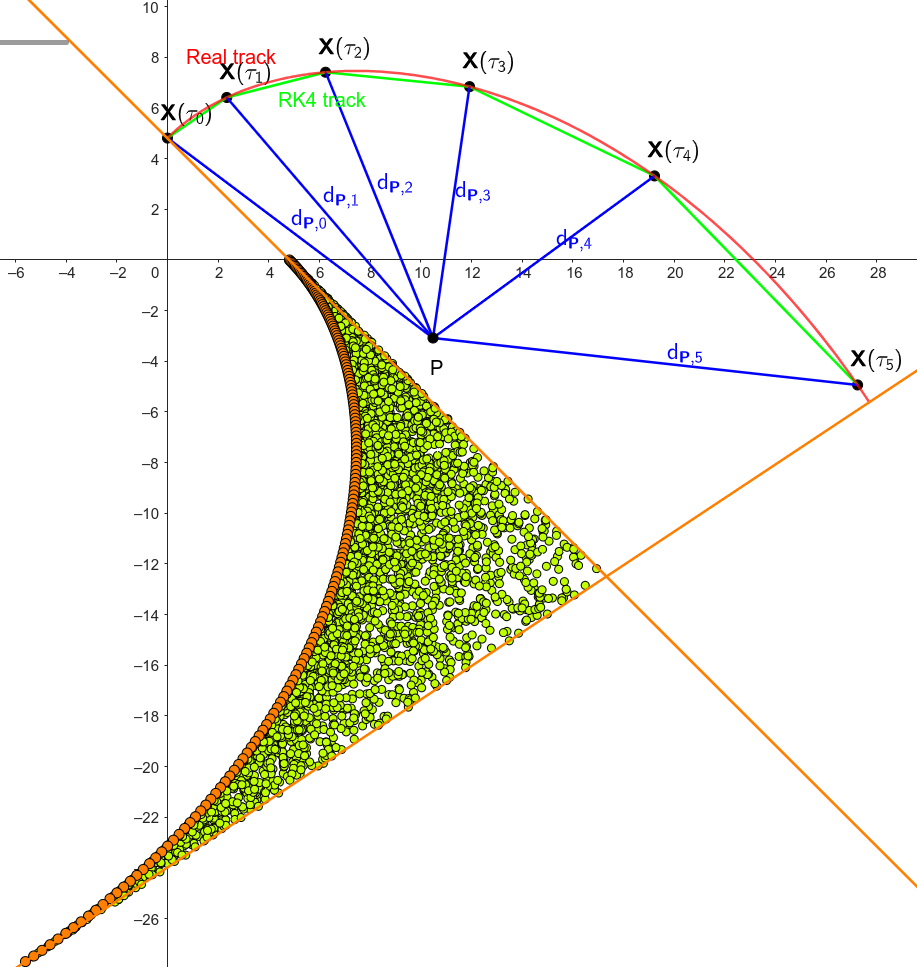
\includegraphics[width=\textwidth]{rk_dist_demo.png}
				\end{subfigure}
				\hfill
				\begin{subfigure}[t]{0.49\textwidth}
					\centering
					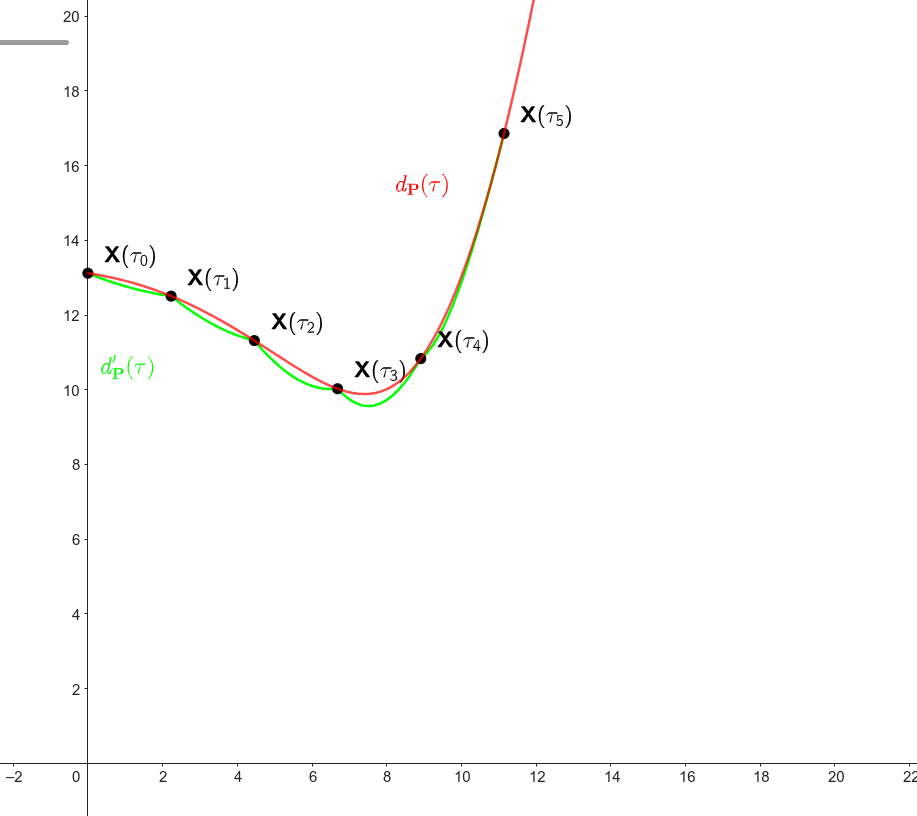
\includegraphics[width=\textwidth]{rk_dist_demo2.png}
				\end{subfigure}
				\hfill
				\begin{subfigure}[t]{0.49\textwidth}
					\centering
					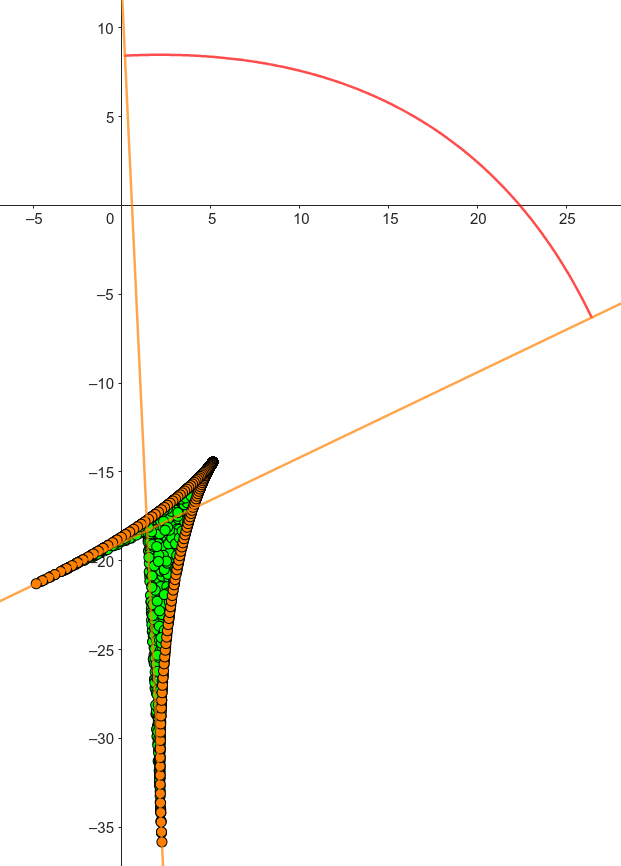
\includegraphics[width=\textwidth]{rk_dist_demo3.png}
				\end{subfigure}
				\caption{\textcolor{red}{some provisional figures}}
				\label{fig:rkdemo2}
			\end{figure}
		
		With the~assumption~\ref{eq:rk_assum}, we can find the~segment on the~\ac{RK4} track with the~lowest distance to a~given point~$\mathbf{P}$ using a~binary search algorithm. Let the~distance of the~point from the $n$\nobreakdash-th vertex %(resp. segment) 
		be~$d_{\mathbf{P},n}$%(resp.~$d_{\mathbf{P},n}'$). For every~$n$, there is a~$\tau_n'\in[\tau_{n-1},\tau_n]$ such that $d_{\mathbf{P}}(\tau_n') = d_{\mathbf{P},n}'$. Since~$d_{\mathbf{P}}(\tau)$ is a~continuous convex function and $\tau \in [0,\tau_N]$ for a~\ac{RK4} track with $N+1$~points, there is a~single minimum $d_{\textbf{P},\text{min}} = d_{\mathbf{P}}(\tau_\text{min})$ for some~$\tau_\text{min}\in[0,\tau_N]$%\in\{\tau_n'\}_{n=1}^N$.\footnote{the~distance to two neighboring segments can be the same if the~closest point is in their common vertex $\tau_n' = \tau_{n+1}'$}
		. Then the difference $\Delta d_{\mathbf{P},n} = d_{\mathbf{P},n}-d_{\mathbf{P},n-1}$ satisfies
			%\begin{equation}
			%	\begin{aligned}
			%		\Delta d_{\mathbf{P},n} &\leq 0\quad \forall n \in \{1,\ldots,k\},\\
			%		\Delta d_{\mathbf{P},n} &\geq 0\quad \forall n \in \{k+1,\ldots,N\}.
			%	\end{aligned}
			%\end{equation}
			\begin{equation}
				\begin{aligned}
					\Delta d_{\mathbf{P},n} &< 0\quad \forall n \text{ such that } \tau_n < \tau_\text{min},\\
					\Delta d_{\mathbf{P},n} &> 0\quad \forall n \text{ such that } \tau_{n-1} > \tau_\text{min}.
				\end{aligned}
			\end{equation}
		Therefore, we can search for the~segment containing $d_{\textbf{P},\text{min}}$ with binary search starting with $\Delta d_{\mathbf{P},1}$ and $\Delta d_{\mathbf{P},N}$, then calculate the~difference $\Delta d_{\mathbf{P},m}$ for the~middle index $m = \left\lfloor\frac{N+1}{2}\right\rfloor$. If $\Delta d_{\mathbf{P},m} > 0$ (\textcolor{red}{minor bug in the implementation -- if the value for the~maximal index is negative, it shouldn't change anything}), we can replace the~higher index with~$m$, otherwise we replace the lower index. The~search stops when the~difference between the~minimal and maximal index is one. \textcolor{red}{Would it be better if they were the same (maybe not)? Then the minimal value is $d_{\mathbf{P},n-1}$ or $d_{\mathbf{P},N}$ and we can take the minimum of the~distances from the~two segments connected to $n-1$. Currently taking the maximal index (and starting at $N-2$ maximal index $\leftrightarrow$ $N-1$\nobreakdash-th point), this should be equivalent, since either $\Delta d_{\mathbf{P},\text{max}} > 0$ (in the code is equivalent to max-1 here) or we are at $N-1$. The minimum of the two distances still taken.}
		
		\textcolor{red}{Same details with MIGRAD etc. as previously.}